\ttlfig{fig:grade_level}{Grade-level Difficulties}{
    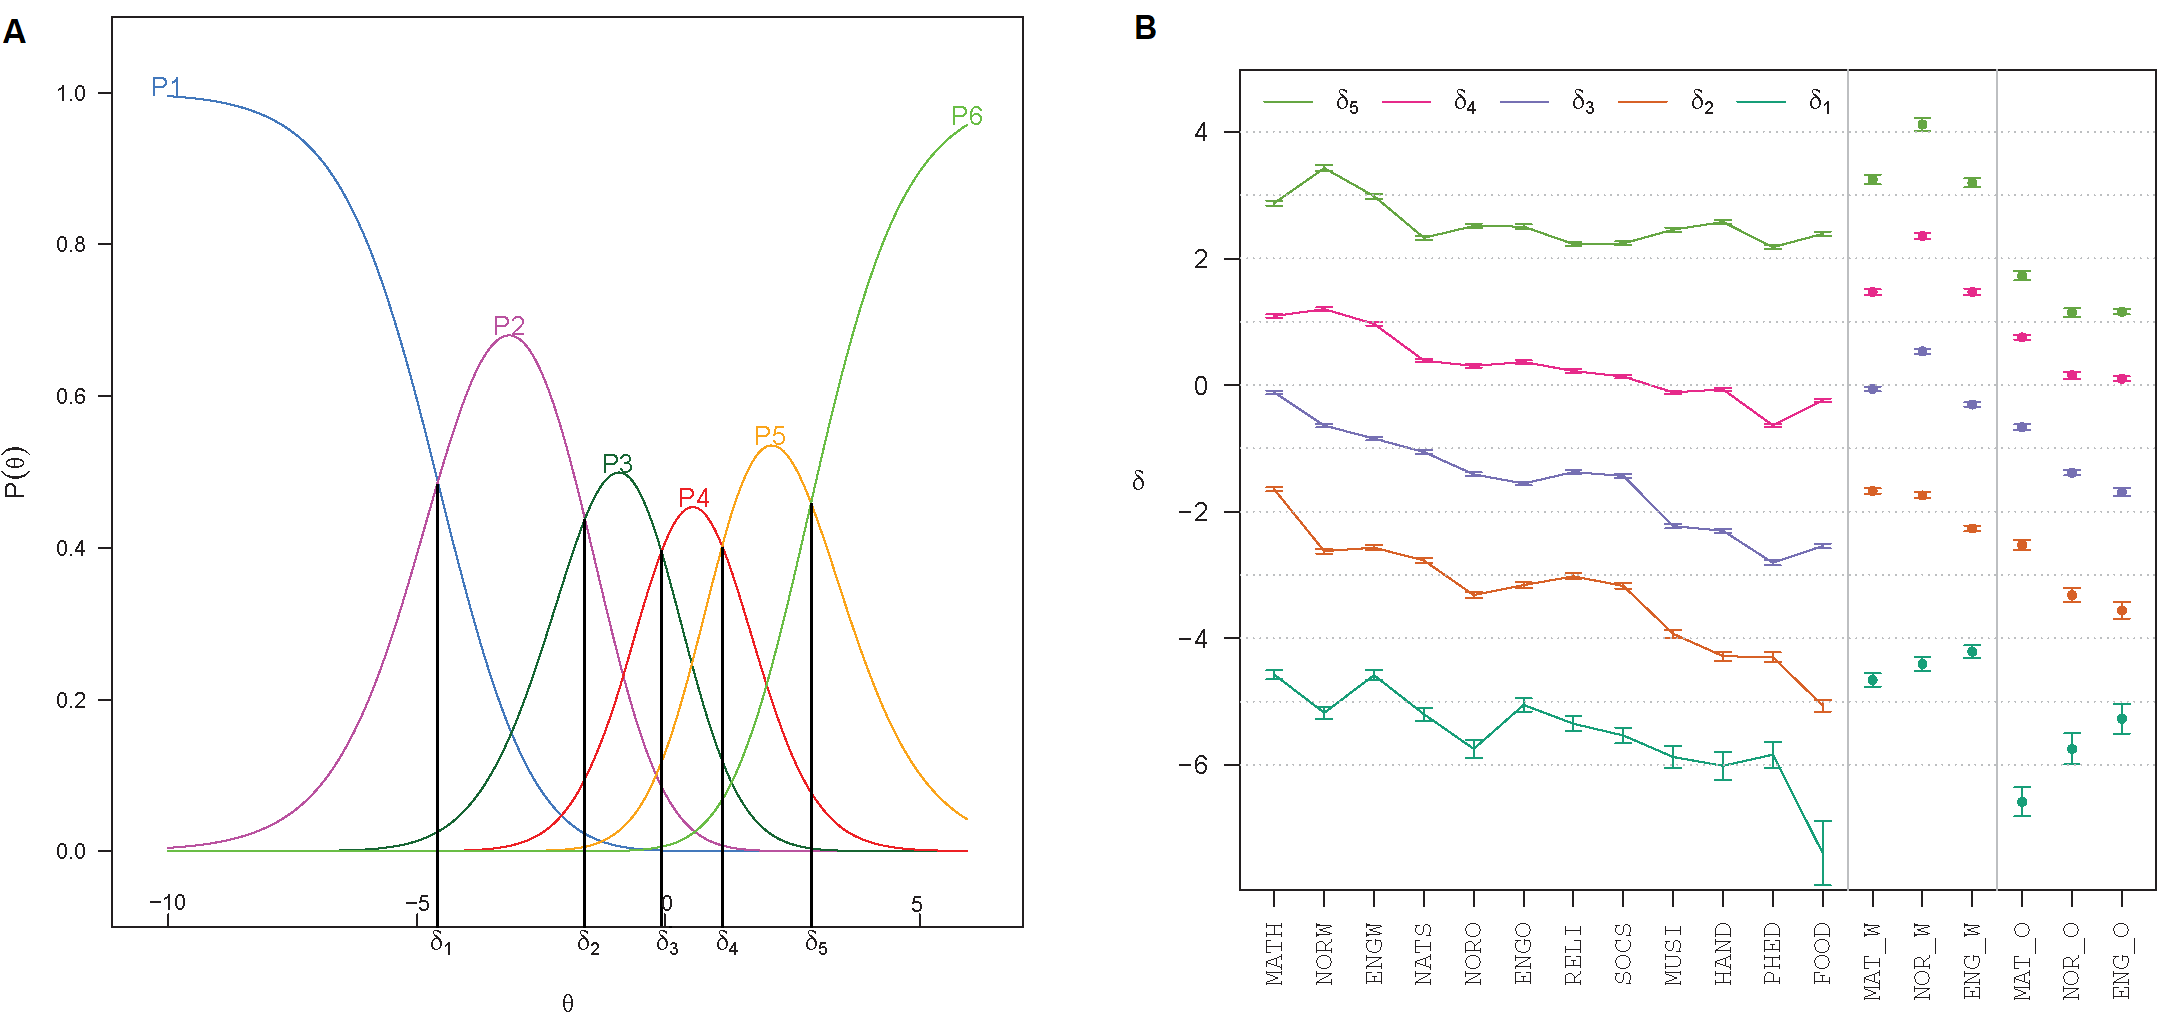
\includegraphics[width=1.5\textwidth]{./Figures/grade_level.png}
}{Panel A illustrates the category characteristic curve (\textsc{ccc}) for \textsc{math}. The vertical axis represents probabilities ranging from $0$ to $1$, and the horizontal axis represents students' latent competencies ranging from low ($\theta=-10$) to high ($\theta=5$). The \textsc{ccc} $P1$, for example, describes the association between competency levels and the likelihood students posessing this competency would receive Grade 1. The intersection between $P1$ and $P2$ marks a difficulty threshold $\delta_1$, above which Grade 2 is a more likely outcome. Six \textsc{ccc}s produce five thresholds $\delta_1, \dots, \delta_5$, which concisely summarise each subject's \emph{grade-level difficulties}. Repeating this procedure to all 18 \textsc{gpa} subjects produces Panel B. The 95\% confidence intervals are pooled over ten imputed datasets.}
